\documentclass[a4paper,oneside,article,11pt]{memoir}

\usepackage[english]{babel}
\usepackage[utf8]{inputenc}
\usepackage{amsmath,amssymb,amsthm}

\newtheorem*{toprove}{At bevise}
\newtheorem{lemma}{Lemma}
\newtheorem{thrm}{Theorem}

% This font looks so good.
\usepackage[sc]{mathpazo}

% Typesetting pseudo-code
\usepackage{algorithm}
\usepackage{algorithmic}
\usepackage{multirow}
% Code comments like [CLRS]
\renewcommand{\algorithmiccomment}[1]{\makebox[5cm][l]{$\triangleright$ \textit{#1}}}
\usepackage{framed,graphicx,xcolor}
\usepackage{listings}

\usepackage[font={small,it}]{caption}

% Relative references
\usepackage{varioref}

\usepackage{tikz}

\bibliographystyle{plain}

\title{Dynamic Algorithms \\ Dynamic Transitive Closure }
\author{Peter Gabrielsen 20114179 \\
Christoffer Hansen 20114637}
\newcounter{qcounter}
\begin{document}

\maketitle
\thispagestyle{empty}
\clearpage
\tableofcontents
\clearpage

\chapter{Introduction}
In this project we look at the dynamic transitive closure problem of a directed unweighted graph $G$.

\begin{itemize}
\item{\texttt{init($n$)}: $G$ becomes the empty directed graph with vertices $\left\lbrace 0,\dots, n-1\right\rbrace$ and no edges.}
\item{\texttt{insert($i,j$)}: Inserts an edge from $i$ to $j$ into $G$ (if it is not already contained in $G$).}
\item{\texttt{delete($i,j$)}: Deletes an edge from $i$ to $j$ from $G$ (if it is contained in $G$).}
\item{\texttt{transitiveClosure?}: Returns the total number of edges in the transitive closure graphs.}
\end{itemize}

We are going to implement two dynamic algorithms for this problem. The first, presented in section~\ref{chap:fw}, is a trivial solution based on the Floyd-Warshall algorithm for computing all pairs shortest paths. The next solution, presented in section~\ref{chap:sankowski}, is based on Sankowski's randomized reduction to dynamic matrix adjoint combined with the use of the Sherman-Morrison formula.

The second solution requires us to do arithmetic modulo a prime $p$. We are thus going to describe algorithms for this in time $\mathcal{O}(\log^2(p))$ in section \ref{chap:prime}.

Finally we are going to experimentally test both algorithms and compare their running time on different inputs interesting to this problem in section~\ref{chap:exp}.


\chapter{Floyd-Warshall}
\label{chap:fw}

Floyd-Warshall's algorithm is an algorithm for finding all-pairs shortest path in a directed graph. The algorithm in its traditional form uses a bottom-up dynamic programming approach to compute the shortest-path weights. It does so using the following recurrence:

$$
d_{ij}^{(k)} = \left\{ \begin{array}{ll}
w_{ij} &\mbox{ if $k=0$} \\
\min\left(d_{ij}^{(k-1)}, d_{ik}^{(k-1)} + d_{kj}^{(k-1)}\right) &\mbox{ if $k \geq 1$}
\end{array} \right.
$$

In the k'th iteration the Floyd-Warshall algorithm considers the shortest path from $i$ to $j$ with intermediate vertices in the set $\left\lbrace 1,2,\dots,k-1\right\rbrace$. It computes the k'th iteration by decomposing the path from $i$ to $j$ into $i \rightsquigarrow k \rightsquigarrow j$. Since $k$ is not an intermediate vertex of the path $i\rightsquigarrow k$ or $k\rightsquigarrow j$ we satisfy having already computed the shortest path of these paths and can easily expand our solution using the recurrence.

We are, however, interested in computing the transitive closure of a directed graph and not all-pairs shortest path, but the Floyd-Warshall algorithm can be easily modified to solve this problem.

We do this by assigning a weight of 1 to each edge in our graph. If there is a path from $i$ to $j$ we will have that $d_{ij} < n$ otherwise $d_{ij} = \infty$. Another approach, which is both more efficient and simpler, is to replace the use of arithmetic operations with logical operations $\wedge$ and $\vee$. The k'th iteration computes whether there is a path from $i$ to $j$ by checking if it already exists or if it exists by considering the path $i\rightsquigarrow k\rightsquigarrow j$. By the same argument as before, we have already computed whether a path exists from $i$ to $k$ and $k$ to $j$. The recurrence becomes:

$$
t_{ij}^{(k)} = \left\{ \begin{array}{ll}
\left\{
\begin{array}{ll}
0 &\mbox{ if $i \neq j $ and $ (i,j)\not\in E$} \\
1 &\mbox{ if $i = j $ and $ (i,j)\in E$}
\end{array} 
\right.
&\mbox{ if $k=0$} \\
t_{ij}^{(k-1)} \vee \left(d_{ik}^{(k-1)} \wedge d_{kj}^{(k-1)}\right) &\mbox{ if $k \geq 1$}
\end{array} \right.
$$

The algorithm for computing the transitive closure using Floyd-Warshall is repeated in algorithm~\ref{alg:fw}. The complexity of this algorithm is trivially $\mathcal{O}(n^3)$ by the triple \texttt{for} loops.

The complexity of each operation is also quite simple. In the lazy solution we only compute the transitive closure when needed and we can thus do \texttt{insert} and \texttt{delete} in $\mathcal{O}(1)$. Using lazy initialization \texttt{init} can be done in $\mathcal{O}(1)$ but our solution simply initializes the adjacency matrix and transitive closure graph upfront using $\mathcal{O}(n^2)$ operations. Finally the transitive closure can be computed in $\mathcal{O}(n^3)$.

Another solution is to eagerly update the transitive closure matrix on each \texttt{insert} and \texttt{delete} giving these operations a complexity of $\mathcal{O}(n^3)$. The complexity of \texttt{init} is the same as for the lazy solution, but we are now able to report number of edges in the transitive closure graph in $\mathcal{O}(1)$.

The complexities are repeated in figure~\ref{fig:fw-comp}.

%algorithm
\begin{algorithm}[h]
\caption{\textsc{Floyd-Warshall Transitive Closure}(Graph $G$)}
\label{alg:fw}
\begin{algorithmic}[1]
\FOR{$k \leftarrow 1 $ to $n$}
	\FOR{$i \leftarrow 1 $ to $n$}
		\FOR{$j \leftarrow 1 $ to $n$}
			\STATE{$G_{ij} = G_{ij} \vee (G_{ik} \wedge G_{kj})$}
		\ENDFOR
	\ENDFOR
\ENDFOR
\end{algorithmic}
\end{algorithm}

\begin{figure}[h]
\center{
\begin{tabular}{|c|c|c|}
\hline
Operation & Lazy & Eager \\\hline
\texttt{init} & $\mathcal{O}(1)$ or $\mathcal{O}(n^2)$ & $\mathcal{O}(1)$ or $\mathcal{O}(n^2)$ \\
\texttt{insert} & $\mathcal{O}(1)$ & $\mathcal{O}(n^3)$ \\
\texttt{delete} & $\mathcal{O}(1)$ & $\mathcal{O}(n^3)$ \\
\texttt{transitiveClosure?} & $\mathcal{O}(n^3)$ & $\mathcal{O}(1)$ \\\hline
\end{tabular}
}
\caption{Complexities of each operation for the Floyd-Warshall solution.}
\label{fig:fw-comp}
\end{figure}

\chapter{Sankowski's randomized dynamic algorithm}
\label{chap:sankowski}

The dynamic algorithm we will present here is due to Sankowski's randomized reduction to dynamic matrix adjoint~\cite{Reif1997347} with use of the Sherman-Morrison formula~\cite{lecnotes}.

Sankowski presents the following theorem in \cite{Reif1997347}, which is the main idea of our proposed algorithm.

\begin{thrm}
\label{thrm:sankowski-path}
Let $A$ be the adjacency matrix of a graph $G$. There exists a path in $G$ from $i$ to $j$ \textit{iff} $adj(I-A)_{ij}$ as polynomial of entries of $A$ is symbolically not equal to zero.
\end{thrm}

Assuming $(I-A)$ is non-singular it trivially follows that $det(I-A) \not = 0$. From the relation $(I-A)^{-1} = \frac{adj(I-A)}{det(I-A)}$ it follows that $(I-A)^{-1}$ could simply be considered as a scaling of $adj(I-A)$ by a scalar corresponding to $\frac{1}{det(I-A)}$. Put in other words, non-zero entries of $adj(I-A)$ is preserved when dividing with $det(I-A)$.

In order to efficiently compute the inverse of the adjacency matrix we look into the Sherman-Morrison formula.

\subsection{Sherman-Morrison formula}

Assume $A$ is an invertible square matrix of size $n \times n$ and $u$, $v$ are column vectors of size $n \times 1$. %TODO We don't need this assumption: For now we will assume that $1 + v^T A^{-1} u \not = 0$.

From the Sherman-Morrison formula,

\begin{equation} \label{eq:ShermanMorrison}
(A+uv^T)^{-1} = A^{-1} - \dfrac{A^{-1}uv^TA^{-1}}{1 + v^T A^{-1} u}
\end{equation}

one may see that we are provided with a numerical cheap way of computing the inverse of $A + uv^T$ under the invariant that we know $A^{-1}$. It is clear that $uv^T$ can be considered as a rank-one update of the matrix $A$.

%TODO Should we show that SM can be computed effeciently?

\subsection{Putting it all together}
The idea of the algorithm is to combine Sankowskis reduction to dynamic matrix adjoint combined with the Sherman-Morrison formula.

Unfortunately we can not rely on a polynomial of degree $n$ as it could take exponential time to evaluate. In order to come around this issue we choose a prime $p$ and for each variable (i.e. non-zero entry of $A$) we substitute with a uniformly random $r \in \mathbb{Z}_{p} := \mathbb{Z} / p\mathbb{Z}$. Thus, the algorithm becomes:

\begin{itemize}
\item{\texttt{init($n$)}: Set $A^{-1}$ = $I_n$. Note that $I_n$ is equal to $(I_n)^{-1}$. Also  initialize a matrix $B^{n \times n}$ taking uniformly random values from $\mathbb{Z}_p$ in all entries.}
\item{\texttt{insert($i,j$)}: If edge does not already exist then let $u = e_i$ be the unit column vector of length $n$ with 1 in entry $i$. Let $v$ be the column vector of length n with all-zeroes expect from entry $j$ that takes it value from $B_{ij}$.
Use the Sherman-Morrison formula presented in Equation~\ref{eq:ShermanMorrison} to compute the inverse $A^{-1}$.}
\item{\texttt{delete($i,j$)}: As \texttt{delete($i,j$)} could simply be viewed as the inverse permutation of A with respect to \texttt{insert($i,j$)}, we change the signs in the Sherman-Morrison formula as follows

$$(A+uv^T)^{-1} = A^{-1} + \dfrac{A^{-1}uv^TA^{-1}}{1 - v^T A^{-1} u}$$

Assuming $u$, $v$ on the same form as in \texttt{insert($i,j$)}, we are ensured having done an inverse permutation of A with respect to \texttt{insert($i,j$)}.

We only delete if the edge has previously been inserted.
}

\item{\texttt{transitiveClosure?}: From Theorem~\ref{thrm:sankowski-path} it follows that we just have to report all non-zero entries of $A^{-1}$.}
\end{itemize}

\subsection{Probability of errors}

Conceptually we want to store a matrix of unique symbols and then the determinant of this matrix would be a polynomial of degree $\leq n$ in at most $n^2$ variables. The symbolic determinant stored would be symbolically equal to zero iff there is no edge from $i$ to $j$. Since all variables are distinct we have that none of the permutation terms can cancel out, and we would be home-free. We can however not afford to evaluate these polynomials so we have to settle for a random matrix modulo a prime $p$.
This introduces so-called false zeros. The determinant of the $n \times n$ random matrix can be seen as a polynomial of degree $\leq n$. The probability of a false zero is bounded in the following lemma ~\ref{lma:zippelSchwarz}.

\begin{lemma}
\label{lma:zippelSchwarz}
If $p(x_1$,...,$x_m)$ is a non-zero polynomial of degree $d$ with coefficients in a field and $S$ is a subset of the field, then the probability that $p$ evaluates to 0 on a random element $(s_1$,$s_2$...,$s_m) \in S^m$ is at most $d/\rvert S \rvert$. We call this event false zero.
\end{lemma}

This gives us that the probability that the determinant of a random $n \times n$ matrix, $B$, modulo $p$ is at most $n/p$.

\begin{align}
\label{error-prob}
Pr\left[ \det(I-B)  = 0\right] \leq \frac{n}{p} \leq \frac{1}{n^{c-1}}
\end{align}
for a prime $p \geq n^c$.

Since we are effectively calculating the adjugate matrix which consists of $n^2$ determinants of $n-1 \times n-1$ matrices we have that the probability of a false zero in one or more of them is given by:

$$Pr\left[ \bigcup\limits_{i,j} adj_{ij}(I-B) = 0\right] \leq \sum\limits_{i,j}Pr\left[adj_{ij}(I-B) = 0\right] \leq \frac{n^3}{p} \leq \frac{1}{n^{c-3}}$$
using the union bound.

If we now want to ensure that for $p = 2^{31}-1$ have an error probability of less than $\frac{1}{n}$ then we will have that $n$ can be at most:
$$\frac{n^3}{2^{31}-1} \leq \frac{1}{n} \Rightarrow n^4 \leq 2^{31}-1 \Rightarrow n \leq (2^{31}-1)^{\frac{1}{4}} \approx 215$$


\subsection{Complexity analysis}

\begin{itemize}
\item{\texttt{init($n$)}: Computing the identity matrix of size $n$ can trivially be done in $\mathcal{O}(n^2)$ time and space. We also need to compute the random matrix $B^{n \times n}$ that takes random values from $\mathbb{Z}_p$. It is assumed that we can choose a uniformly random $k$-bit number in time $\mathcal{O}(k)$. Thus it takes $\mathcal{O}(n^2 log(p))$ to initialize $B$. Note that we can use lazy initialization to get an $\mathcal{O}(1)$ running time.}
\item{\texttt{insert($i,j$)}: The Sherman-Morrison takes $\mathcal{O}(n^2)$ to evaluate. We assume, for now, arithmetic operations can be done in $O(\log^2(p))$ per operation in $\mathbb{Z}_p$. This gives a total running time of $\mathcal{O}(n^2 \log^2(p))$.}
\item{\texttt{delete($i,j$)}: Same analysis as \texttt{insert($i,j$)} gives $\mathcal{O}(n^2 \log^2(p))$.}
\item{\texttt{transitiveClosure?}: We run through the entire matrix $A^{-1}$ yielding an $\mathcal{O}(n^2)$ traversal to report.}
\end{itemize}

All results are repeated in~Figure~\ref{fig:truly-comp}.

\begin{figure}[h]
\center{
\begin{tabular}{|c|c|c|}
\hline
Operation & Normal initialization & Lazy initialization \\\hline
\texttt{init} & $\mathcal{O}(n^2 \log p)$ & $\mathcal{O}(1)$ \\
\texttt{insert} & $\mathcal{O}(n^2 \log^2 p)$ & $\mathcal{O}(n^2 \log^2 p)$ \\
\texttt{delete} & $\mathcal{O}(n^2 \log^2 p)$ & $\mathcal{O}(n^2 \log^2 p)$ \\
\texttt{transitiveClosure?} & $\mathcal{O}(n^2)$ & $\mathcal{O}(n^2)$ \\\hline
\end{tabular}
}
\caption{Complexities of each operation for the truly dynamic solution.}
\label{fig:truly-comp}
\end{figure}

\chapter{Implementation}
\label{impl}

We implemented both dynamic algorithms described in section~\ref{chap:fw} and section~\ref{chap:sankowski}. For the prime needed in the algorithm described in section~\ref{chap:sankowski}, we used $p = 2^{31}-1$ as it has the advantage that we can do all operations within double precision arithmetic.



\chapter{Arithmetic modulo $p$}
\label{chap:prime}
In order to achieve the bounds presented in section~\ref{chap:sankowski} we need to be able to do fast arithmetic operations modulo $p$. There we used that the operations can be performed in $\mathcal{O}(\log^2(p))$. This is trivially true for all operations except division, since they are simply the normal operation followed by a modulo operation.

We cannot just use normal division when in $\mathbb{Z}/p\mathbb{Z}$. We need to compute the multiplicative inverse of the denominator and multiply this with the numerator modulo $p$. We need to show that the multiplicative inverse can be computed in $\mathcal{O}(\log^2(p))$. We will do this using the extended euclidean algorithm. In addition to computing the greatest common divisor $d$ of $a$ and $b$, the extended euclidean algorithm also computes $x$ and $y$ such that $d = ax+by$ (Bézout's identity). If we compute this identity with $b = p$ we have that $1 = ax+py$, since the greatest common divisor of $a$ and $p$ will always be $1$ in the field $\mathbb{Z}/p\mathbb{Z}$, i.e. all elements have an inverse. Now the modular inverse of $a$ is simply $x$ modulo $p$ since $py = 0$ in the field. Lets sum up these results in algorithm~\ref{alg:modinv} for computing the modular inverse modulo $p$.

%algorithm
\begin{algorithm}[H]
\caption{\textsc{Extended-Euclid}(a,b)}
\label{alg:extended_euclidean}
\begin{algorithmic}[1]
\IF{$b=0$}
	\RETURN{$(a,1,0)$}
\ELSE
	\STATE{$(d',x',y') = \textsc{Extended-Euclid}(b,\, a \mod b)$}
	\STATE{$(d,x,y) = (d',y',x'-\lfloor a/b \rfloor y')$}
	\RETURN{$(d,x,y)$}
\ENDIF
\end{algorithmic}
\end{algorithm}

%algorithm
\begin{algorithm}[H]
\caption{\textsc{Modulo Inverse}(a,b)}
\label{alg:modinv}
\begin{algorithmic}[1]
\STATE{$(d,x,y) = \textsc{Extended-Euclid}(a,b)$}
\IF{$d > 1$}
	\STATE{No inverse exists}
\ELSE
	\RETURN{$x \mod b$}
\ENDIF
\end{algorithmic}
\end{algorithm}

We see that the complexity is bounded by the complexity of computing the greatest common divisor in the extended euclidean algorithm.

\subsection{The running time of the Extended Euclidean algorithm}
The running time of this algorithm is equal to the number of recursive calls we make. The worst case analysis makes use of Fibonacci numbers, since calculating the greatest common divisor of two consecutive Fibonacci numbers will produce the worst case number of recursive calls.
The analysis is similar to the one given in~\cite[p.~935-937]{clrs}.

The following lemma gives a condition on the size of the input in order to perform $k \geq 1$ recursive calls.

\begin{lemma}
\label{lemma:ee-rec}
If $a > b \geq 1$ and the call to \textsc{Extended-Euclid}(a,b) performs $k \geq 1$ recursive calls, then $a \geq F_{k+2}$ and $b \geq F_{k+1}$.
\end{lemma}
\begin{proof}
The proof is by induction on $k$.

The basis of the induction is $k=1$. Then we must have that $b \geq 1 = F_2$ and $a > b \Rightarrow a \geq 2 = F_3$. By the construction of Fibonacci numbers we have that $b > (a \mod b)$, which implies that, in each recursive call the first argument is strictly larger than the second.

Now assume that the lemma holds for $k-1$ recursive calls. We are now going to prove that it holds for $k$ recursive calls. We have that $b > 0$ and that \textsc{Extended-Euclid}(a,b) calls \textsc{Extended-Euclid}(b, a mod b) recursively, which by the induction hypothesis makes $k-1$ recursive calls. The induction hypothesis also tells us that $b \geq F_{k+1}$ and $a \mod b \geq F_k$.

We have that:
\begin{align*}
b+(a\mod b) &= b + (a-b\lfloor a/b \rfloor) \\
&\leq a
\end{align*}
since $a > b > 0 \Rightarrow \lfloor a/b \rfloor \geq 1$. It now follows that:
\begin{align*}
a &\geq b + (a \mod b) \\
&\geq F_{k+1} + F_k \\
&= F_{k+2}
\end{align*}
\end{proof}

Lamés theorem follows directly from lemma~\ref{lemma:ee-rec} and says that for any integer $k\geq 1$, if $a > b \geq 1$ and $b < F_{k+1}$, then the number of recursive calls is less than $k$.

It can be shown that the upper bound achieved from Lamés theorem is the best possible by looking at the call to \textsc{Extended-Euclid}($F_{k+1}$, $F_k$). By induction on $k$ we see that we will need $k-1$ recursive calls.
The inductive step is as follows:
\begin{align*}
\gcd(F_{k+1}, F_k) &= \gcd(F_k, F_{k+1} \mod F_k)\\
&= \gcd(F_k, F_{k-1})
\end{align*}

Since $F_k = \Theta(\phi^k)$ where $\phi$ is the golden ratio we have that the number of recursive calls is $\mathcal{O}(\lg_{\phi} b) = \mathcal{O}(\lg b)$. We perform a constant number of $\mathcal{O}(\lg p)$ arithmetic operations in each recursive call and we thus achieve a total complexity of $\mathcal{O}(\lg^2 p)$ for division modulo $p$.

\chapter{Experiments}
\label{chap:exp}
In this section we are going to test our two algorithms on various input to test the correctness and running time under different conditions.

\subsection{Correctness}
We tested correctness of our algorithms by computing the transitive closure on the given test data and then compare the results using the \texttt{diff} tool. It was however not feasible to compute the transitive closure on the $1000 \times 1000$ matrix using Floyd-Warshall's algorithm, but the algorithms computed the same results on the other given input data.

\subsection{Running time on given test data}
We tested the algorithms' running time by running the given tests and measuring the running time. Since the number of operations vary significantly in the tests we normalized the data by dividing the running time with the number of operations, giving the running time per operation as a function of $n$. The data was fitted to $f(x) = ax^3$ and $f(x)=ax^2\log_2 x$ for Floyd-Warshall's and Sankowski's respectively.

The results are depicted in figure~\ref{fig:norm-run-comb}. We see that the data can be fitted to the curves with a large constant factor.
\begin{figure}[ht]
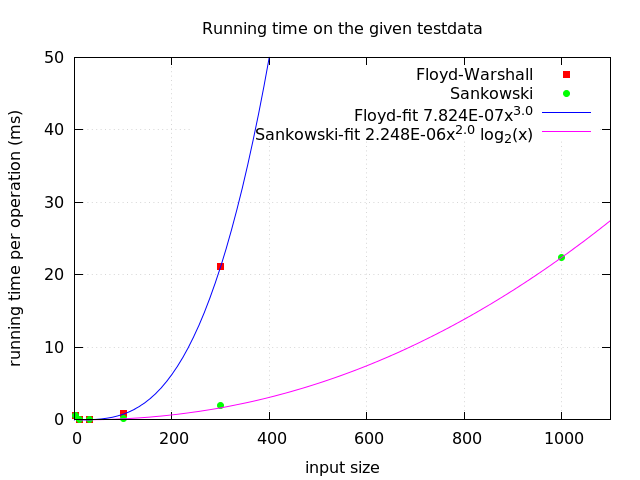
\includegraphics[width=\textwidth]{images/normalized-given-data-running.png}
\caption{Running time of the given data normalized by number of operations}
\label{fig:norm-run-comb}
\end{figure}

\subsection{Running time}
We wanted to tighter result than the one we were able to give from the given test data, so we constructed another experiment to test the running time of our algorithms. We set $p=2^{31}-1$ and the test was $5000$ \texttt{insert}'s, $5000$ \texttt{delete}'s uniformly distributed and a call to \texttt{transitiveClosure?} between every other operation, i.e. $10000$ \texttt{transitiveClosure?} calls. Then we let $n$ go from $10$ to $300$ with a step size of $10$. The results are depicted in figure~\ref{fig:running}. It is plotted as running time per operation divided by $n^2$. This should give us a logarithmic curve for Sankowski's randomized solution and a linear curve for the solution based on Floyd-Warshall's.

\begin{figure}[ht]
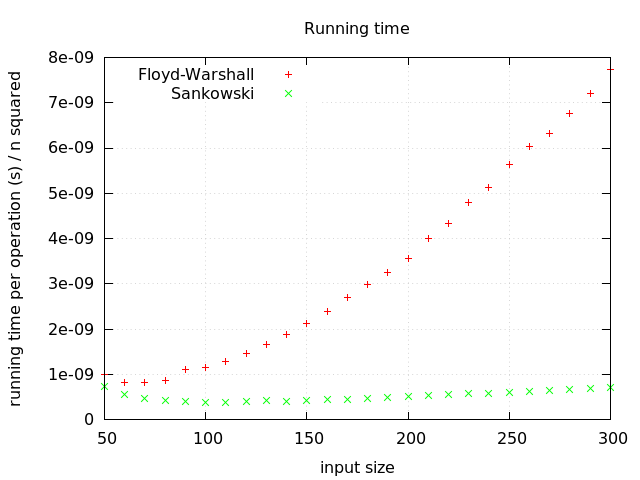
\includegraphics[width=\textwidth]{images/running-time-GOOD.png}
\caption{Running time for Floyd-Warshall's and Sankowski's respectively.}
\label{fig:running}
\end{figure}

\subsection{Error probability}
We experimented with the error probability introduced in Sankowski's randomized dynamic solution. The experiment counted the number of \texttt{insert} and \texttt{delete} operations possible before introducing an error into the transitive closure matrix. We did this by repeatedly filling and emptying an $100 \times 100$ matrix until the results from Floyd-Warshall's and Sankowski's solution did not match. For each prime number we repeated the experiment 10 times and averaged the result. We expect that the result is linear in the size of $p$ from equation~\ref{error-prob}.
\begin{figure}[ht]
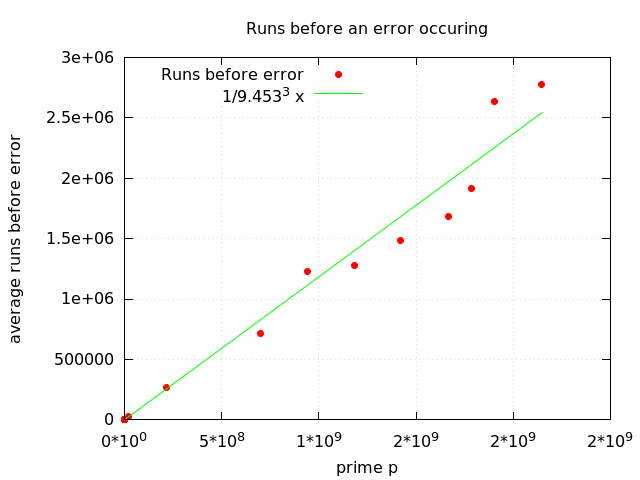
\includegraphics[width=\textwidth]{images/error-probability2.png}
\caption{Number of runs before an error}
\label{fig:num-runs}
\end{figure}

\bibliography{references}
\end{document}


